% questions.tex —— 2011 年·重庆卷·理科 · 题目内容片段（无答案）
% 由 tools/generate_projects.py 依来源总账自 2011/2011_数学真题_重庆理_试题.md 生成，勿手改（改源 MD 后重跑）

\gkpart{一、选择题}

\begin{question}
\gkti{1}复数 $\dfrac{\mathrm i^2+\mathrm i^3+\mathrm i^4}{1-\mathrm i}=$\mbox{（　　）}

（A）$-\frac12-\frac12\mathrm i$

（B）$-\frac12+\frac12\mathrm i$

（C）$\frac12-\frac12\mathrm i$

（D）$\frac12+\frac12\mathrm i$

\end{question}
\begin{question}
\gkti{2}“$x<-1$”是“$x^2-1>0$”的\mbox{（　　）}

（A）充分而不必要条件

（B）必要而不充分条件

（C）充要条件

（D）既不充分也不必要条件

\end{question}
\begin{question}
\gkti{3}已知 $\lim\limits_{x\to\infty}\left(\dfrac2{x-1}+\dfrac{ax-1}{3x}\right)=2$，则 $a=$\mbox{（　　）}

（A）$-6$

（B）$2$

（C）$3$

（D）$6$

\end{question}
\begin{question}
\gkti{4}$(1+3x)^n$（其中 $n\in\mathbf N$ 且 $n\geqslant6$）的展开式中 $x^5$ 与 $x^6$ 的系数相等，则 $n=$\mbox{（　　）}

（A）$6$

（B）$7$

（C）$8$

（D）$9$

\end{question}
\begin{question}
\gkti{5}下列区间中，函数 $f(x)=|\ln(2-x)|$ 在其上为增函数的是\mbox{（　　）}

（A）$(-\infty,1]$

（B）$\left[-1,\frac43\right]$

（C）$\left[0,\frac32\right)$

（D）$[1,2)$

\end{question}
\begin{question}
\gkti{6}若 $\triangle ABC$ 的内角 $A$，$B$，$C$ 所对的边 $a$，$b$，$c$ 满足 $(a+b)^2-c^2=4$，且 $C=60^\circ$，则 $ab$ 的值为\mbox{（　　）}

（A）$\frac43$

（B）$8-4\sqrt3$

（C）$1$

（D）$\frac23$

\end{question}
\begin{question}
\gkti{7}已知 $a>0$，$b>0$，$a+b=2$，则 $y=\dfrac1a+\dfrac4b$ 的最小值是\mbox{（　　）}

（A）$\frac72$

（B）$4$

（C）$\frac92$

（D）$5$

\end{question}
\begin{question}
\gkti{8}在圆 $x^2+y^2-2x-6y=0$ 内，过点 $E(0,1)$ 的最长弦和最短弦分别为 $AC$ 和 $BD$，则四边形 $ABCD$ 的面积为\mbox{（　　）}

（A）$5\sqrt2$

（B）$10\sqrt2$

（C）$15\sqrt2$

（D）$20\sqrt2$

\end{question}
\begin{question}
\gkti{9}高为 $\dfrac{\sqrt2}4$ 的四棱锥 $S-ABCD$ 的底面是边长为 $1$ 的正方形，点 $S$，$A$，$B$，$C$，$D$ 均在半径为 $1$ 的同一球面上，则底面 $ABCD$ 的中心与顶点 $S$ 之间的距离为\mbox{（　　）}

（A）$\frac{\sqrt2}4$

（B）$\frac{\sqrt2}2$

（C）$1$

（D）$\sqrt2$

\end{question}
\begin{question}
\gkti{10}设 $m$，$k$ 为整数，方程 $mx^2-kx+2=0$ 在区间 $(0,1)$ 内有两个不同的根，则 $m+k$ 的最小值为\mbox{（　　）}

（A）$-8$

（B）$8$

（C）$12$

（D）$13$

\end{question}
\gkpart{二、填空题}

\begin{question}
\gkti{11}在等差数列 $\{a_n\}$ 中，$a_3+a_7=37$，则 $a_2+a_4+a_6+a_8=\underline{\qquad}$。

\end{question}
\begin{question}
\gkti{12}已知单位向量 $\boldsymbol e_1$，$\boldsymbol e_2$ 的夹角为 $60^\circ$，则 $|2\boldsymbol e_1-\boldsymbol e_2|=\underline{\qquad}$。

\end{question}
\begin{question}
\gkti{13}将一枚均匀的硬币抛掷 $6$ 次，则正面出现的次数比反面出现的次数多的概率为 $\underline{\qquad}$。

\end{question}
\begin{question}
\gkti{14}已知 $\sin\alpha=\dfrac12+\cos\alpha$，且 $\alpha\in\left(0,\dfrac\pi2\right)$，则 $\dfrac{\cos2\alpha}{\sin\left(\alpha-\dfrac\pi4\right)}$ 的值为 $\underline{\qquad}$。

\end{question}
\begin{question}
\gkti{15}设圆 $C$ 位于抛物线 $y^2=2x$ 与直线 $x=3$ 所围成的封闭区域（包含边界）内，则圆 $C$ 的半径能取到的最大值为 $\underline{\qquad}$。

\end{question}
\gkpart{三、解答题}

\begin{question}
\gkti{16}设 $a\in\mathbf R$，$f(x)=\cos x(a\sin x-\cos x)+\cos^2\left(\dfrac\pi2-x\right)$ 满足 $f\left(-\dfrac\pi3\right)=f(0)$，求函数 $f(x)$ 在 $\left[\dfrac\pi4,\dfrac{11\pi}{24}\right]$ 上的最大值和最小值。

\end{question}
\begin{question}
\gkti{17}某市公租房的房源位于 $A$，$B$，$C$ 三个片区。设每位申请人只申请其中一个片区的房源，且申请其中任一个片区的房源是等可能的。求该市的任 $4$ 位申请人中：

（1） 恰有 $2$ 人申请 $A$ 片区的房源的概率；

（2） 申请的房源所在片区的个数 $\xi$ 的分布列与期望。

\end{question}
\begin{question}
\gkti{18}设 $f(x)=x^3+ax^2+bx+1$ 的导数 $f'(x)$ 满足 $f'(1)=2a$，$f'(2)=-b$，其中常数 $a$，$b\in\mathbf R$。

（1） 求曲线 $y=f(x)$ 在点 $(1,f(1))$ 处的切线方程；

（2） 设 $g(x)=f'(x)\mathrm e^{-x}$，求函数 $g(x)$ 的极值。

\Needspace{0.4\textheight}
\end{question}
\begin{question}
\gkti{19}如图，在四面体 $ABCD$ 中，平面 $ABC\perp$ 平面 $ACD$，$AB\perp BC$，$AD=CD$，$\angle CAD=30^\circ$。

（1） 若 $AD=2$，$AB=2BC$，求四面体 $ABCD$ 的体积；

（2） 若二面角 $C-AB-D$ 为 $60^\circ$，求异面直线 $AD$ 与 $BC$ 所成角的余弦值。
\nopagebreak[4]
\begin{center}% 2011 年重庆卷理科第 19 题：四面体 ABCD，平面 ABC⊥平面 ACD。
% 来源 PDF：普通高考/2011/2011重庆理.pdf，SHA-256 15c5e4dfbc23f3b3e1c37b279db7aea1a8e3db05ea86087e2346208274bc7ef7。
% 原页：第 2 页第 1 栏上部，书页码 652。示意。
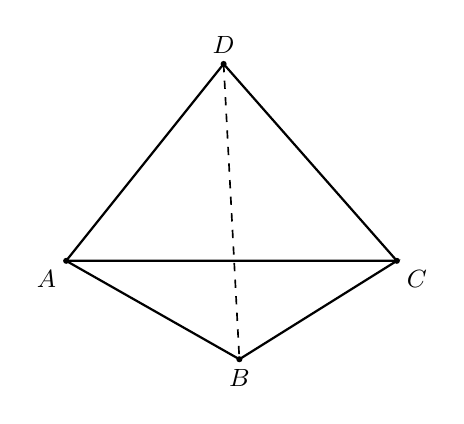
\begin{tikzpicture}[>=stealth, semithick, font=\small, scale=1.0]
  \coordinate (A) at (0,0);
  \coordinate (C) at (4.2,0);
  \coordinate (B) at (2.2,-1.25);
  \coordinate (D) at (2.0,2.5);
  \draw[thick] (A)--(B)--(C)--(A);
  \draw[thick] (D)--(A) (D)--(C);
  \draw[dashed] (D)--(B);
  \fill (A) circle (1.1pt) node[below left] {$A$};
  \fill (B) circle (1.1pt) node[below] {$B$};
  \fill (C) circle (1.1pt) node[below right] {$C$};
  \fill (D) circle (1.1pt) node[above] {$D$};
\end{tikzpicture}
\end{center}
\nopagebreak[4]
\Needspace{0.4\textheight}
\end{question}
\begin{question}
\gkti{20}如图，椭圆的中心为原点 $O$，离心率 $e=\dfrac{\sqrt2}2$，一条准线的方程为 $x=2\sqrt2$。

（1） 求该椭圆的标准方程；

（2） 设动点 $P$ 满足 $\overrightarrow{OP}=\overrightarrow{OM}+2\overrightarrow{ON}$，其中 $M$，$N$ 是椭圆上的点，直线 $OM$ 与 $ON$ 的斜率之积为 $-\dfrac12$。问：是否存在两个定点 $F_1$，$F_2$，使得 $|PF_1|+|PF_2|$ 为定值？若存在，求 $F_1$，$F_2$ 的坐标；若不存在，说明理由。
\nopagebreak[4]
\begin{center}% 2011 年重庆卷理科第 20 题：椭圆、准线 x=2√2 与点 P、M、N。
% 来源 PDF：普通高考/2011/2011重庆理.pdf，SHA-256 15c5e4dfbc23f3b3e1c37b279db7aea1a8e3db05ea86087e2346208274bc7ef7。
% 原页：第 2 页第 2 栏中部，书页码 652。示意。
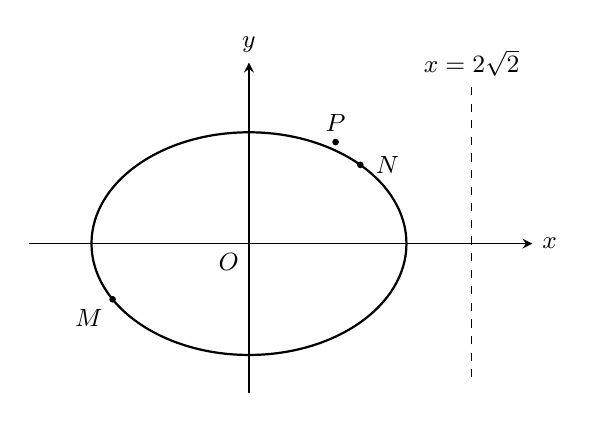
\begin{tikzpicture}[>=stealth, semithick, font=\small, scale=1.0]
  \draw[->] (-2.8,0)--(3.6,0) node[right] {$x$};
  \draw[->] (0,-1.9)--(0,2.3) node[above] {$y$};
  \draw[thick] (0,0) ellipse (2 and 1.414);
  \draw[dashed] (2.828,-1.7)--(2.828,2.0) node[above] {$x=2\sqrt2$};
  \fill (-1.732,-0.707) circle (1.2pt) node[below left] {$M$};
  \fill (1.414,1.0) circle (1.2pt) node[right=2pt] {$N$};
  \fill (1.10,1.29) circle (1.2pt) node[above] {$P$};
  \node[below left] at (0,0) {$O$};
\end{tikzpicture}
\end{center}
\nopagebreak[4]
\end{question}
\begin{question}
\gkti{21}设实数数列 $\{a_n\}$ 的前 $n$ 项和 $S_n$ 满足 $S_{n+1}=a_{n+1}S_n$（$n\in\mathbf N^*$）。

（1） 若 $a_1$，$S_2$，$-2a_2$ 成等比数列，求 $S_2$ 和 $a_3$；

（2） 求证：对 $k\geqslant3$ 有 $0\leqslant a_{k+1}\leqslant a_k\leqslant\dfrac43$。

\end{question}